\chapter{Puukyselyt}

Tyypillisiä puukyselyitä ovat
puun polkuihin ja alipuihin
liittyvät kyselyt.
Tämä luku esittelee
tekniikoita, joiden avulla on mahdollista
toteuttaa puukyselyjä tehokkaasti.
Usein esiintyvä idea on muuttaa
puu jollakin tavalla taulukoksi,
mikä helpottaa puun käsittelyä.

\section{Tehokas nouseminen}

\begin{task}
Annettuna on juurellinen puu, jonka solmut on numeroitu
$1 \ldots n$ ja juurisolmu on 1.
Tehtäväsi on vastata
kyselyihin muotoa ''mikä solmu on
$k$ askelta ylempänä solmua $s$''.
\end{task}

Merkitään $f(s,k)$ solmua,
joka on $k$ askelta ylempänä solmua $s$.
Esimerkiksi seuraavassa puussa
$f(2,1)=1$ ja $f(8,2)=4$.

\begin{center}
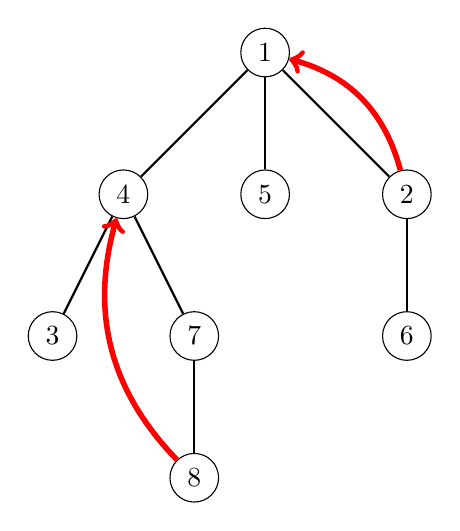
\begin{tikzpicture}[scale=0.9]
\node[draw, circle] (1) at (0,3) {$1$};
\node[draw, circle] (2) at (2,1) {$2$};
\node[draw, circle] (3) at (-2,1) {$4$};
\node[draw, circle] (4) at (0,1) {$5$};
\node[draw, circle] (5) at (2,-1) {$6$};
\node[draw, circle] (6) at (-3,-1) {$3$};
\node[draw, circle] (7) at (-1,-1) {$7$};
\node[draw, circle] (8) at (-1,-3) {$8$};
\path[draw,thick,-] (1) -- (2);
\path[draw,thick,-] (1) -- (3);
\path[draw,thick,-] (1) -- (4);
\path[draw,thick,-] (2) -- (5);
\path[draw,thick,-] (3) -- (6);
\path[draw,thick,-] (3) -- (7);
\path[draw,thick,-] (7) -- (8);

\path[draw=red,thick,->,line width=2pt] (8) edge [bend left] (3);
\path[draw=red,thick,->,line width=2pt] (2) edge [bend right] (1);
\end{tikzpicture}
\end{center}

Suoraviivainen tapa laskea funktion $f(s,k)$
arvo on kulkea puussa $k$ askelta ylöspäin
solmusta $s$ alkaen.
Tämän aikavaativuus on kuitenkin $O(n)$,
koska on mahdollista, että puussa on alaspäin
kulkeva ketju, jossa on $O(n)$ solmua.

Funktion $f(s,k)$ arvo on kuitenkin mahdollista
laskea ajassa $O(\log n)$ sopivan esilaskennan avulla.
Jokaiseen solmuun $s$ lasketaan
etukäteen kaikki arvot
$f(s,k)$, joissa $k=1,2,4,8,\ldots$ eli 2:n potenssi.
Tämän jälkeen mikä tahansa askelmäärä $k$
muodostuu $O(\log n)$ esilasketusta arvosta.

Kun $k=1$, arvot $f(s,k)$ on helppo laskea,
koska riittää mennä yksi kaari ylemmäs.
Kun taas $k>1$, pätee kaava
$f(s,k)=f(f(s,k/2),k/2)$, eli $k$ askeleen
nousun pystyy jakamaan kahdeksi $k/2$
askeleen nousuksi.
Esimerkiksi äskeisessä puussa $f(8,1)=7$
ja $f(7,1)=4$, joten $f(8,2)=f(f(8,1),1)=4$.

Esilasketut arvot vievät tilaa $O(n \log n)$,
ja niiden avulla pystyy vastaamaan
mihin tahansa kyselyyn ajassa $O(\log n)$.

\section{Alipuiden käsittely}

\begin{task}
Annettuna on juurellinen puu, jossa on $n$ solmua.
Jokaisen solmun väri on sininen tai punainen.
Tehtäväsi on käsitellä kyselyt muotoa
''muuta solmun $s$ väriä'' sekä
''montako sinistä solmua on
solmun $s$ alipuussa''.
\end{task}

Esimerkiksi puussa
\begin{center}
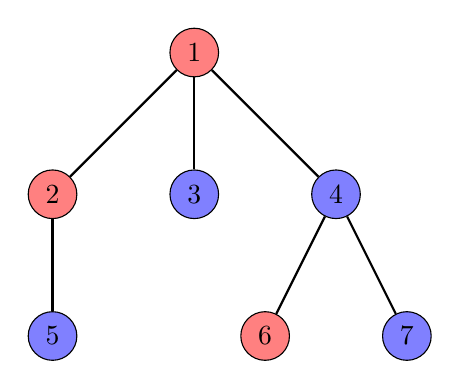
\begin{tikzpicture}[scale=0.9]
\definecolor{lightblue}{rgb}{0.5,0.5,1}
\definecolor{lightred}{rgb}{1,0.5,0.5}

\node[draw, circle, fill=lightred] (1) at (0,3) {$1$};
\node[draw, circle, fill=lightred] (2) at (-2,1) {$2$};
\node[draw, circle, fill=lightblue] (3) at (2,1) {$4$};
\node[draw, circle, fill=lightblue] (4) at (0,1) {$3$};
\node[draw, circle, fill=lightblue] (5) at (-2,-1) {$5$};
\node[draw, circle, fill=lightblue] (6) at (3,-1) {$7$};
\node[draw, circle, fill=lightred] (7) at (1,-1) {$6$};
\path[draw,thick,-] (1) -- (2);
\path[draw,thick,-] (1) -- (3);
\path[draw,thick,-] (1) -- (4);
\path[draw,thick,-] (2) -- (5);
\path[draw,thick,-] (3) -- (6);
\path[draw,thick,-] (3) -- (7);
\end{tikzpicture}
\end{center}
solmun 1 alipuussa on 4 sinistä solmua,
solmun 2 alipuussa on 1 sininen solmu
ja solmun 4 alipuussa on 2 sinistä solmua.

Alipuiden käsittelyssä kätevä tekniikka on
järjestää solmut sen mukaan,
missä järjestyksessä puun juuresta lähtevä
syvyyshaku vierailee solmuissa.
Tällöin jokaiseen alipuuhun
kuuluvat solmut ovat vierekkäin järjestyksessä.
Esimerkkipuussa syvyyshaku etenee
\begin{center}
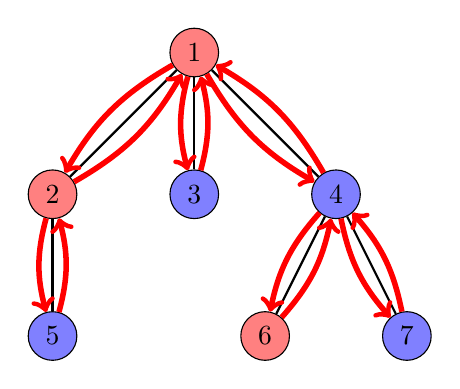
\begin{tikzpicture}[scale=0.9]
\definecolor{lightblue}{rgb}{0.5,0.5,1}
\definecolor{lightred}{rgb}{1,0.5,0.5}

\node[draw, circle, fill=lightred] (1) at (0,3) {$1$};
\node[draw, circle, fill=lightred] (2) at (-2,1) {$2$};
\node[draw, circle, fill=lightblue] (3) at (2,1) {$4$};
\node[draw, circle, fill=lightblue] (4) at (0,1) {$3$};
\node[draw, circle, fill=lightblue] (5) at (-2,-1) {$5$};
\node[draw, circle, fill=lightblue] (6) at (3,-1) {$7$};
\node[draw, circle, fill=lightred] (7) at (1,-1) {$6$};
\path[draw,thick,-] (1) -- (2);
\path[draw,thick,-] (1) -- (3);
\path[draw,thick,-] (1) -- (4);
\path[draw,thick,-] (2) -- (5);
\path[draw,thick,-] (3) -- (6);
\path[draw,thick,-] (3) -- (7);

\path[draw=red,thick,->,line width=2pt] (1) edge [bend right=15] (3);
\path[draw=red,thick,->,line width=2pt] (3) edge [bend right=15] (6);
\path[draw=red,thick,->,line width=2pt] (6) edge [bend right=15] (3);
\path[draw=red,thick,->,line width=2pt] (3) edge [bend right=15] (7);
\path[draw=red,thick,->,line width=2pt] (7) edge [bend right=15] (3);
\path[draw=red,thick,->,line width=2pt] (3) edge [bend right=15] (1);
\path[draw=red,thick,->,line width=2pt] (1) edge [bend right=15] (4);
\path[draw=red,thick,->,line width=2pt] (4) edge [bend right=15] (1);
\path[draw=red,thick,->,line width=2pt] (1) edge [bend right=15] (2);
\path[draw=red,thick,->,line width=2pt] (2) edge [bend right=15] (5);
\path[draw=red,thick,->,line width=2pt] (5) edge [bend right=15] (2);
\path[draw=red,thick,->,line width=2pt] (2) edge [bend right=15] (1);
\end{tikzpicture}
\end{center}
ja tuottaa järjestyksen
\begin{center}
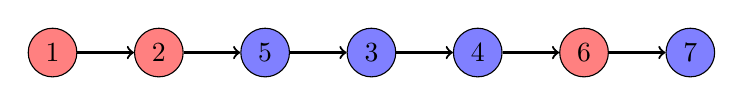
\begin{tikzpicture}[scale=0.9]
\definecolor{lightblue}{rgb}{0.5,0.5,1}
\definecolor{lightred}{rgb}{1,0.5,0.5}

\node[draw, circle, fill=lightred] (1) at (0,0) {$1$};
\node[draw, circle, fill=lightred] (2) at (1.5,0) {$2$};
\node[draw, circle, fill=lightblue] (4) at (6,0) {$4$};
\node[draw, circle, fill=lightblue] (3) at (4.5,0) {$3$};
\node[draw, circle, fill=lightblue] (5) at (3,0) {$5$};
\node[draw, circle, fill=lightblue] (7) at (9,0) {$7$};
\node[draw, circle, fill=lightred] (6) at (7.5,0) {$6$};
\path[draw,thick,->] (1) -- (2);
\path[draw,thick,->] (2) -- (5);
\path[draw,thick,->] (5) -- (3);
\path[draw,thick,->] (3) -- (4);
\path[draw,thick,->] (4) -- (6);
\path[draw,thick,->] (6) -- (7);
\end{tikzpicture}
\end{center}

Ideana on tallentaa tietoa solmuista taulukoihin
syvyyshaun järjestyksessä.
Tässä tehtävässä tarvittavat taulukot ovat
\texttt{node}, \texttt{size} ja \texttt{color}.
Taulukossa \texttt{node} on solmujen tunnukset,
taulukossa \texttt{size} on alipuiden solmujen määrät
ja taulukossa \texttt{color} on solmujen värit
(0 = punainen, 1 = sininen).

Esimerkkipuussa taulukot ovat seuraavat:
\begin{center}
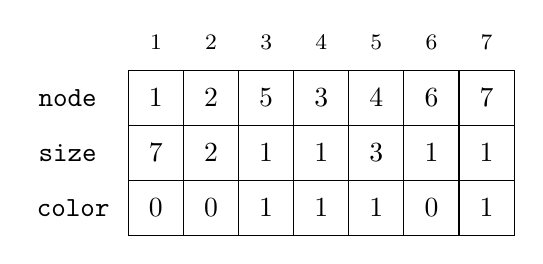
\begin{tikzpicture}[scale=0.7]
\draw (0,1) grid (7,2);
\node at (-1.1,1.5) {\texttt{node}};
\node at (0.5,1.5) {$1$};
\node at (1.5,1.5) {$2$};
\node at (2.5,1.5) {$5$};
\node at (3.5,1.5) {$3$};
\node at (4.5,1.5) {$4$};
\node at (5.5,1.5) {$6$};
\node at (6.5,1.5) {$7$};

\draw (0,0) grid (7,1);
\node at (-1.1,0.5) {\texttt{size}};
\node at (0.5,0.5) {$7$};
\node at (1.5,0.5) {$2$};
\node at (2.5,0.5) {$1$};
\node at (3.5,0.5) {$1$};
\node at (4.5,0.5) {$3$};
\node at (5.5,0.5) {$1$};
\node at (6.5,0.5) {$1$};

\draw (0,-1) grid (7,0);
\node at (-1,-0.5) {\texttt{color}};
\node at (0.5,-0.5) {$0$};
\node at (1.5,-0.5) {$0$};
\node at (2.5,-0.5) {$1$};
\node at (3.5,-0.5) {$1$};
\node at (4.5,-0.5) {$1$};
\node at (5.5,-0.5) {$0$};
\node at (6.5,-0.5) {$1$};

\footnotesize
\node at (0.5,2.5) {$1$};
\node at (1.5,2.5) {$2$};
\node at (2.5,2.5) {$3$};
\node at (3.5,2.5) {$4$};
\node at (4.5,2.5) {$5$};
\node at (5.5,2.5) {$6$};
\node at (6.5,2.5) {$7$};
\end{tikzpicture}
\end{center}

Taulukoiden avulla voi laskea
sinisten solmujen määrän minkä tahansa solmun $s$ alipuussa.
Ideana on etsiä taulukosta \texttt{node}
kohta $x$, jossa $\texttt{node}[x]=s$.
Tämän jälkeen $\texttt{size}[x]$ kertoo solmun $s$
alipuun solmujen määrän ja alipuun solmujen
värit ovat $\texttt{color}[x]$,$\texttt{color}[x+1]$,$\texttt{color}[x+2]$, jne.
Alipuun solmut ovat aina peräkkäin taulukoissa,
koska solmut ovat syvyyshaun järjestyksessä.

Lasketaan esimerkkinä sinisten solmujen määrä solmun 4
alipuussa:

\begin{center}
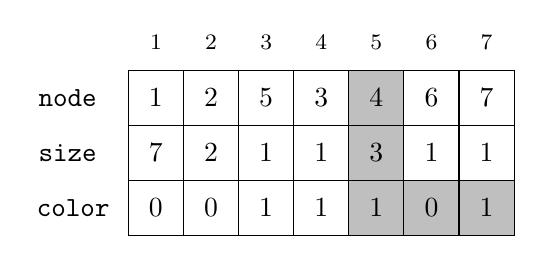
\begin{tikzpicture}[scale=0.7]
\fill[color=lightgray] (4,1) rectangle (5,2);
\fill[color=lightgray] (4,0) rectangle (5,1);
\fill[color=lightgray] (4,-1) rectangle (7,0);

\draw (0,1) grid (7,2);
\node at (-1.1,1.5) {\texttt{node}};
\node at (0.5,1.5) {$1$};
\node at (1.5,1.5) {$2$};
\node at (2.5,1.5) {$5$};
\node at (3.5,1.5) {$3$};
\node at (4.5,1.5) {$4$};
\node at (5.5,1.5) {$6$};
\node at (6.5,1.5) {$7$};

\draw (0,0) grid (7,1);
\node at (-1.1,0.5) {\texttt{size}};
\node at (0.5,0.5) {$7$};
\node at (1.5,0.5) {$2$};
\node at (2.5,0.5) {$1$};
\node at (3.5,0.5) {$1$};
\node at (4.5,0.5) {$3$};
\node at (5.5,0.5) {$1$};
\node at (6.5,0.5) {$1$};

\draw (0,-1) grid (7,0);
\node at (-1,-0.5) {\texttt{color}};
\node at (0.5,-0.5) {$0$};
\node at (1.5,-0.5) {$0$};
\node at (2.5,-0.5) {$1$};
\node at (3.5,-0.5) {$1$};
\node at (4.5,-0.5) {$1$};
\node at (5.5,-0.5) {$0$};
\node at (6.5,-0.5) {$1$};

\footnotesize
\node at (0.5,2.5) {$1$};
\node at (1.5,2.5) {$2$};
\node at (2.5,2.5) {$3$};
\node at (3.5,2.5) {$4$};
\node at (4.5,2.5) {$5$};
\node at (5.5,2.5) {$6$};
\node at (6.5,2.5) {$7$};
\end{tikzpicture}
\end{center}

Taulukosta \texttt{node} selviää,
että solmu 4 on kohdassa 5 syvyyshaun
järjestyksessä.
Sitten taulukko \texttt{size} kertoo,
että solmun alipuussa on 3 solmua,
ja lopulta taulukko \texttt{color}
sisältää solmujen värit.
Sinisten solmujen määrä solmun 4
alipuussa on taulukon \texttt{color}
välin summa eli $1+0+1=2$.

Solmun sijainti taulukossa \texttt{node}
selviää ajassa $O(1)$ tallentamalla
sijainnit käänteiseen taulukkoon.
Taulukon \texttt{color} muuttaminen ja
välin summan laskenta onnistuvat ajassa $O(\log n)$
tekemällä segmenttipuu, jossa on taulukon sisältö.
Niinpä molemmat kyselyt on mahdollista toteuttaa
ajassa $O(\log n)$.

\section{Alin yhteinen esivanhempi}

Juurellisessa puussa kahden solmun $a$ ja $b$
alin yhteinen esivanhempi (\textit{lowest common ancestor})
on mahdollisimman alhaalla puussa oleva solmu,
jonka alipuussa ovat molemmat solmut $a$ ja $b$.
Luonteva tehtävä on:

\begin{task}
Annettuna on juurellinen puu, jossa on $n$ solmua.
Tehtäväsi on vastata kyselyihin
''mikä on solmujen $a$ ja $b$ alin yhteinen esivanhempi''.
\end{task}


\begin{samepage}
Esimerkiksi puussa

\begin{center}
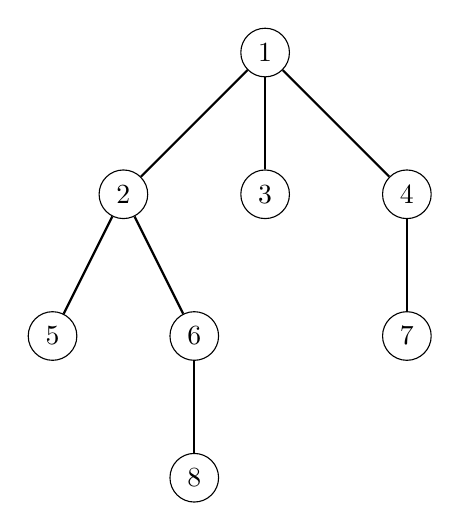
\begin{tikzpicture}[scale=0.9]
\node[draw, circle] (1) at (0,3) {$1$};
\node[draw, circle] (2) at (2,1) {$4$};
\node[draw, circle] (3) at (-2,1) {$2$};
\node[draw, circle] (4) at (0,1) {$3$};
\node[draw, circle] (5) at (2,-1) {$7$};
\node[draw, circle] (6) at (-3,-1) {$5$};
\node[draw, circle] (7) at (-1,-1) {$6$};
\node[draw, circle] (8) at (-1,-3) {$8$};
\path[draw,thick,-] (1) -- (2);
\path[draw,thick,-] (1) -- (3);
\path[draw,thick,-] (1) -- (4);
\path[draw,thick,-] (2) -- (5);
\path[draw,thick,-] (3) -- (6);
\path[draw,thick,-] (3) -- (7);
\path[draw,thick,-] (7) -- (8);
\end{tikzpicture}
\end{center}
\end{samepage}

solmujen 5 ja 8 alin yhteinen esivanhempi on solmu 2
ja solmujen 3 ja 4 alin yhteinen esivanhempi on solmu 1.

Ideana on jälleen järjestää solmut syvyyshaun mukaan:

\begin{center}
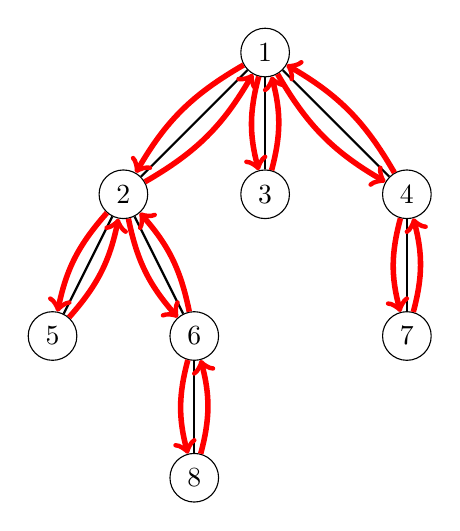
\begin{tikzpicture}[scale=0.9]
\node[draw, circle] (1) at (0,3) {$1$};
\node[draw, circle] (2) at (2,1) {$4$};
\node[draw, circle] (3) at (-2,1) {$2$};
\node[draw, circle] (4) at (0,1) {$3$};
\node[draw, circle] (5) at (2,-1) {$7$};
\node[draw, circle] (6) at (-3,-1) {$5$};
\node[draw, circle] (7) at (-1,-1) {$6$};
\node[draw, circle] (8) at (-1,-3) {$8$};
\path[draw,thick,-] (1) -- (2);
\path[draw,thick,-] (1) -- (3);
\path[draw,thick,-] (1) -- (4);
\path[draw,thick,-] (2) -- (5);
\path[draw,thick,-] (3) -- (6);
\path[draw,thick,-] (3) -- (7);
\path[draw,thick,-] (7) -- (8);

\path[draw=red,thick,->,line width=2pt] (1) edge [bend right=15] (3);
\path[draw=red,thick,->,line width=2pt] (3) edge [bend right=15] (6);
\path[draw=red,thick,->,line width=2pt] (6) edge [bend right=15] (3);
\path[draw=red,thick,->,line width=2pt] (3) edge [bend right=15] (7);
\path[draw=red,thick,->,line width=2pt] (7) edge [bend right=15] (8);
\path[draw=red,thick,->,line width=2pt] (8) edge [bend right=15] (7);
\path[draw=red,thick,->,line width=2pt] (7) edge [bend right=15] (3);
\path[draw=red,thick,->,line width=2pt] (3) edge [bend right=15] (1);
\path[draw=red,thick,->,line width=2pt] (1) edge [bend right=15] (4);
\path[draw=red,thick,->,line width=2pt] (4) edge [bend right=15] (1);
\path[draw=red,thick,->,line width=2pt] (1) edge [bend right=15] (2);
\path[draw=red,thick,->,line width=2pt] (2) edge [bend right=15] (5);
\path[draw=red,thick,->,line width=2pt] (5) edge [bend right=15] (2);
\path[draw=red,thick,->,line width=2pt] (2) edge [bend right=15] (1);
\end{tikzpicture}
\end{center}

Erona aiempaan solmu lisätään kuitenkin järjestykseen
mukaan \textit{aina}, kun syvyyshaku käy solmussa,
eikä vain ensimmäisellä kerralla.
Niinpä solmu esiintyy järjestyksessä $x+1$ kertaa,
missä $x$ on solmun lasten määrä,
ja järjestyksessä on yhteensä $2n-1$ solmua.

Tässä tehtävässä tarvittavat taulukot ovat \texttt{node},
joka sisältää solmujen tunnukset,
sekä \texttt{depth}, jossa on kunkin solmun syvyys puussa.
Juuren syvyys on 1, seuraavan tason solmujen syvyys on 2, jne.

Esimerkkipuuta vastaavat taulukot ovat:

\begin{center}
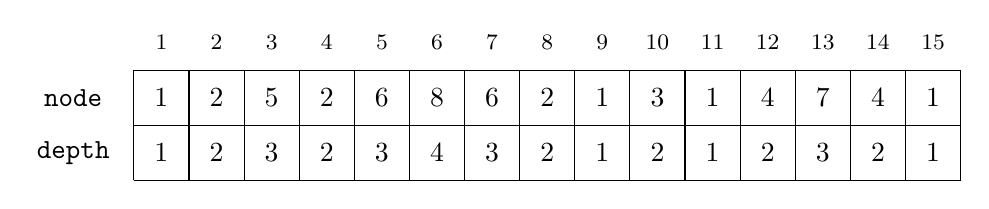
\begin{tikzpicture}[scale=0.7]
%\fill[color=lightgray] (4,1) rectangle (5,2);
%\fill[color=lightgray] (4,0) rectangle (5,1);
%\fill[color=lightgray] (4,-1) rectangle (7,0);

\draw (0,1) grid (15,2);
\node at (-1.1,1.5) {\texttt{node}};
\node at (0.5,1.5) {$1$};
\node at (1.5,1.5) {$2$};
\node at (2.5,1.5) {$5$};
\node at (3.5,1.5) {$2$};
\node at (4.5,1.5) {$6$};
\node at (5.5,1.5) {$8$};
\node at (6.5,1.5) {$6$};
\node at (7.5,1.5) {$2$};
\node at (8.5,1.5) {$1$};
\node at (9.5,1.5) {$3$};
\node at (10.5,1.5) {$1$};
\node at (11.5,1.5) {$4$};
\node at (12.5,1.5) {$7$};
\node at (13.5,1.5) {$4$};
\node at (14.5,1.5) {$1$};


\draw (0,0) grid (15,1);
\node at (-1.1,0.5) {\texttt{depth}};
\node at (0.5,0.5) {$1$};
\node at (1.5,0.5) {$2$};
\node at (2.5,0.5) {$3$};
\node at (3.5,0.5) {$2$};
\node at (4.5,0.5) {$3$};
\node at (5.5,0.5) {$4$};
\node at (6.5,0.5) {$3$};
\node at (7.5,0.5) {$2$};
\node at (8.5,0.5) {$1$};
\node at (9.5,0.5) {$2$};
\node at (10.5,0.5) {$1$};
\node at (11.5,0.5) {$2$};
\node at (12.5,0.5) {$3$};
\node at (13.5,0.5) {$2$};
\node at (14.5,0.5) {$1$};

\footnotesize
\node at (0.5,2.5) {$1$};
\node at (1.5,2.5) {$2$};
\node at (2.5,2.5) {$3$};
\node at (3.5,2.5) {$4$};
\node at (4.5,2.5) {$5$};
\node at (5.5,2.5) {$6$};
\node at (6.5,2.5) {$7$};
\node at (7.5,2.5) {$8$};
\node at (8.5,2.5) {$9$};
\node at (9.5,2.5) {$10$};
\node at (10.5,2.5) {$11$};
\node at (11.5,2.5) {$12$};
\node at (12.5,2.5) {$13$};
\node at (13.5,2.5) {$14$};
\node at (14.5,2.5) {$15$};
\end{tikzpicture}
\end{center}

Näiden taulukoiden avulla solmujen $a$ ja $b$ alin yhteinen esivanhempi
selviää etsimällä taulukosta \texttt{node}
kohdat $x$ ja $y$, joissa $\texttt{node}[x]=a$
ja $\texttt{node}[y]=b$.
Tämän jälkeen taulukon \texttt{depth}
pienin arvo välillä $x \ldots y$
(tai välillä $y \ldots x$, jos $y<x$)
ilmaisee solmun, joka on $a$:n ja $b$:n
alin yhteinen esivanhempi.
Jos on monta vaihtoehtoa valita solmut
$x$ ja $y$, mikä tahansa valinta kelpaa.

Esimerkiksi solmujen 5 ja 8 alin yhteinen esivanhempi
löytyy seuraavasti:

\begin{center}
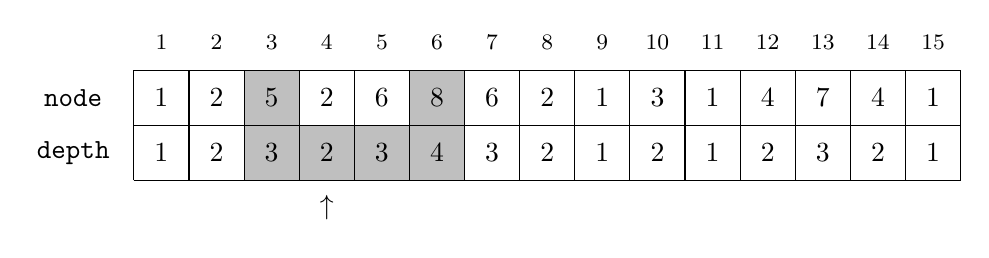
\begin{tikzpicture}[scale=0.7]
\fill[color=lightgray] (2,1) rectangle (3,2);
\fill[color=lightgray] (5,1) rectangle (6,2);
\fill[color=lightgray] (2,0) rectangle (6,1);

\node at (3.5,-0.5) {$\uparrow$};

%\fill[color=lightgray] (4,0) rectangle (5,1);
%\fill[color=lightgray] (4,-1) rectangle (7,0);

\draw (0,1) grid (15,2);
\node at (-1.1,1.5) {\texttt{node}};
\node at (0.5,1.5) {$1$};
\node at (1.5,1.5) {$2$};
\node at (2.5,1.5) {$5$};
\node at (3.5,1.5) {$2$};
\node at (4.5,1.5) {$6$};
\node at (5.5,1.5) {$8$};
\node at (6.5,1.5) {$6$};
\node at (7.5,1.5) {$2$};
\node at (8.5,1.5) {$1$};
\node at (9.5,1.5) {$3$};
\node at (10.5,1.5) {$1$};
\node at (11.5,1.5) {$4$};
\node at (12.5,1.5) {$7$};
\node at (13.5,1.5) {$4$};
\node at (14.5,1.5) {$1$};


\draw (0,0) grid (15,1);
\node at (-1.1,0.5) {\texttt{depth}};
\node at (0.5,0.5) {$1$};
\node at (1.5,0.5) {$2$};
\node at (2.5,0.5) {$3$};
\node at (3.5,0.5) {$2$};
\node at (4.5,0.5) {$3$};
\node at (5.5,0.5) {$4$};
\node at (6.5,0.5) {$3$};
\node at (7.5,0.5) {$2$};
\node at (8.5,0.5) {$1$};
\node at (9.5,0.5) {$2$};
\node at (10.5,0.5) {$1$};
\node at (11.5,0.5) {$2$};
\node at (12.5,0.5) {$3$};
\node at (13.5,0.5) {$2$};
\node at (14.5,0.5) {$1$};

\footnotesize
\node at (0.5,2.5) {$1$};
\node at (1.5,2.5) {$2$};
\node at (2.5,2.5) {$3$};
\node at (3.5,2.5) {$4$};
\node at (4.5,2.5) {$5$};
\node at (5.5,2.5) {$6$};
\node at (6.5,2.5) {$7$};
\node at (7.5,2.5) {$8$};
\node at (8.5,2.5) {$9$};
\node at (9.5,2.5) {$10$};
\node at (10.5,2.5) {$11$};
\node at (11.5,2.5) {$12$};
\node at (12.5,2.5) {$13$};
\node at (13.5,2.5) {$14$};
\node at (14.5,2.5) {$15$};
\end{tikzpicture}
\end{center}

Taulukosta \texttt{node} selviää,
että $\texttt{node}[3]=5$ ja 
$\texttt{node}[6]=8$.
Taulukossa \texttt{depth}
pienin arvo välillä $3 \ldots 6$
on $\texttt{depth}[4]=2$.
Niinpä kohdan 4 solmu eli
solmu 2 on solmujen 5 ja 8
alin yhteinen esivanhempi.

Välin pienin arvo taulukosta \texttt{depth}
selviää tehokkaasti ajassa $O(\log n)$
segmenttipuun avulla.
Koska taulukko ei muutu koskaan,
minimin haku on mahdollista toteuttaa
myös ajassa $O(1)$, mutta tälle on harvoin tarvetta.

\subsubsection{Solmujen etäisyydet}

Myös seuraava tehtävä palautuu alimman yhteisen
esivanhemman hakuun:
\begin{task}
Annettuna on juurellinen puu, jonka solmut on numeroitu $1 \ldots n$.
Tehtäväsi on vastata kyselyihin
''laske solmujen $a$ ja $b$ etäisyys puussa''.
\end{task}

Valitaan ensin mikä tahansa
solmu puun juureksi.
Tämän jälkeen solmujen $a$ ja $b$
etäisyys on $d(a)+d(b)-2 \cdot d(c)$,
missä $c$ on solmujen alin yhteinen esivanhempi
ja $d(s)$ on etäisyys puun juuresta solmuun $s$.
Esimerkiksi puussa

\begin{center}
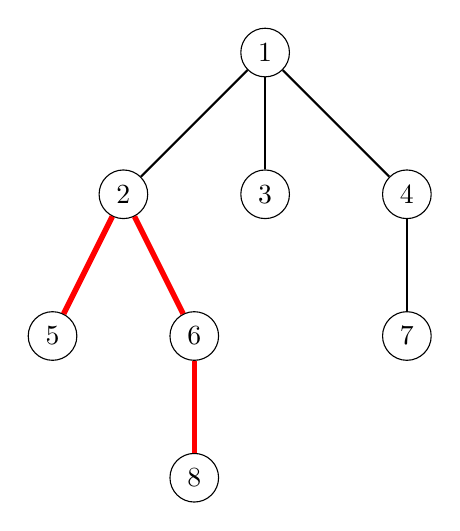
\begin{tikzpicture}[scale=0.9]
\node[draw, circle] (1) at (0,3) {$1$};
\node[draw, circle] (2) at (2,1) {$4$};
\node[draw, circle] (3) at (-2,1) {$2$};
\node[draw, circle] (4) at (0,1) {$3$};
\node[draw, circle] (5) at (2,-1) {$7$};
\node[draw, circle] (6) at (-3,-1) {$5$};
\node[draw, circle] (7) at (-1,-1) {$6$};
\node[draw, circle] (8) at (-1,-3) {$8$};
\path[draw,thick,-] (1) -- (2);
\path[draw,thick,-] (1) -- (3);
\path[draw,thick,-] (1) -- (4);
\path[draw,thick,-] (2) -- (5);
\path[draw,thick,-] (3) -- (6);
\path[draw,thick,-] (3) -- (7);
\path[draw,thick,-] (7) -- (8);

\path[draw=red,thick,-,line width=2pt] (8) -- node[font=\small] {} (7);
\path[draw=red,thick,-,line width=2pt] (7) -- node[font=\small] {} (3);
\path[draw=red,thick,-,line width=2pt] (6) -- node[font=\small] {} (3);
\end{tikzpicture}
\end{center}

solmujen 5 ja 8 alin yhteinen esivanhempi on 2.
Polku solmusta 5 solmuun 8
kulkee ensin ylöspäin solmusta 5
solmuun 2 ja sitten alaspäin
solmusta 2 solmuun 8.
Solmujen etäisyydet juuresta ovat $d(5)=3$,
$d(8)=4$ ja $d(2)=2$,
joten solmujen 5 ja 8 etäisyys
on $3+4-2\cdot2=3$.
